\documentclass[11pt,letterpaper]{article}
\usepackage[top=3cm, bottom=2cm, left=2cm, right=2cm, columnsep=20pt]{geometry}
\usepackage{pdfpages}
\usepackage{graphicx}
\usepackage{etoolbox}
\apptocmd{\sloppy}{\hbadness 10000\relax}{}{}
% \usepackage[numbers]{natbib}
\usepackage[T1]{fontenc}
\usepackage{ragged2e}
\usepackage[french]{babel}
\usepackage{listings}
\usepackage{color}
\usepackage{soul}
\usepackage[utf8]{inputenc}
\usepackage[export]{adjustbox}
\usepackage{caption}
\usepackage{amsmath}
\usepackage{amssymb}
\usepackage{float}
\usepackage{csquotes}
\usepackage{fancyhdr}
\usepackage{wallpaper}
\usepackage{siunitx}
\usepackage[indent]{parskip}
\usepackage{textcomp}
\usepackage{gensymb}
\usepackage{multirow}
\usepackage[hidelinks]{hyperref}
\usepackage{abstract}
\renewcommand{\abstractnamefont}{\normalfont\bfseries}
\renewcommand{\abstracttextfont}{\normalfont\itshape}
\usepackage{titlesec}
\titleformat{\section}{\large\bfseries}{\thesection}{1em}{}
\titleformat{\subsection}{\normalsize\bfseries}{\thesubsection}{1em}{}
\titleformat{\subsubsection}{\normalsize\bfseries}{\thesubsubsection}{1em}{}

\usepackage{xcolor}
\definecolor{codegreen}{rgb}{0,0.6,0}
\definecolor{codegray}{rgb}{0.5,0.5,0.5}
\definecolor{codepurple}{rgb}{0.58,0,0.82}
\definecolor{backcolour}{rgb}{0.95,0.95,0.92}
\lstdefinestyle{mystyle}{
    backgroundcolor=\color{backcolour},   
    commentstyle=\color{codegreen},
    keywordstyle=\color{magenta},
    numberstyle=\tiny\color{codegray},
    stringstyle=\color{codepurple},
    basicstyle=\ttfamily\footnotesize,
    breakatwhitespace=false,         
    breaklines=true,                 
    captionpos=b,                    
    keepspaces=true,                 
    numbers=left,                    
    numbersep=5pt,                  
    showspaces=false,                
    showstringspaces=false,
    showtabs=false,                  
    tabsize=2
}
\lstset{style=mystyle}

\usepackage[most]{tcolorbox}
\newtcolorbox{note}[1][]{
  enhanced jigsaw,
  borderline west={2pt}{0pt}{black},
  sharp corners,
  boxrule=0pt, 
  fonttitle={\large\bfseries},
  coltitle={black},
  title={Note:\ },
  attach title to upper,
  #1
}

%----------------------------------------------------

\setlength{\parindent}{0pt}
\DeclareCaptionLabelFormat{mycaptionlabel}{#1 #2}
\captionsetup[figure]{labelsep=colon}
\captionsetup{labelformat=mycaptionlabel}
\captionsetup[figure]{name={Figure }}
\newcommand{\inlinecode}{\normalfont\texttt}
\usepackage{enumitem}
\setlist[itemize]{label=\textbullet}

\begin{document}
\begin{titlepage}
\center

\begin{figure}
    \ThisULCornerWallPaper{.4}{Polytechnique_signature-RGB-gauche_FR.png}
\end{figure}
\vspace*{2 cm}

\textsc{\Large \textbf{PHS2223 --} Introduction à l'optique moderne}\\[0.5cm]
\large{\textbf{Équipe : 04}}\\[1.5cm]

\rule{\linewidth}{0.5mm} \\[0.5cm]
\Large{\textbf{Expérience 1}} \\[0.2cm]
\text{Microscopie confocale}\\
\rule{\linewidth}{0.2mm} \\[2.3cm]

\large{\textbf{Présenté à}\\
  Guillaume Sheehy\\
  Esmat Zamani\\[2.5cm]
  \textbf{Par :}\\
  Émile \textbf{Guertin-Picard} (2208363)\\
  Laura-Li \textbf{Gilbert} (2204234)\\
  Tom \textbf{Dessauvages} (???????)\\[3cm]}

\large{\today\\
Département de Génie Physique\\
Polytechnique Montréal\\}

\end{titlepage}

%----------------------------------------------------

\tableofcontents
\pagenumbering{roman}
\newpage

\pagestyle{fancy}
\setlength{\headheight}{14pt}
\renewcommand{\headrulewidth}{0pt}
\fancyfoot[R]{\thepage}

\pagestyle{fancy}
\fancyhf{}
\renewcommand{\headrulewidth}{1pt}
\fancyhead[L]{\textbf{PHS2223}}
\fancyhead[C]{Microscopie confocale}
\fancyhead[R]{\today}
\fancyfoot[R]{\thepage}

\pagenumbering{arabic}
\setcounter{page}{1}

%----------------------------------------------------

\section{Introduction}

\section{Théorie}
\subsection{Microsopie Confocale}
La microscopie confocale est une technique d'imagerie avancée qui permet l'obtention d'images à hautes résolution, en éliminant la lumière hors-focus, particulièrement ceux à l'extérieur du plan focal. Le fonctionnement de cette technologie repose sur les principes d'illumination et de détection limités à un certain volume par la présence d'un simple trou, nommé sténopé \textcolor{red}{(Source 1)}. En d'autres termes, ces microscopes fonctionnent de la même manière que ceux conventionnels à l'exception de ce trou. De cette manière, une source de lumière, telle qu'un laser, est émise à travers le système, et celle-ci est, ensuite, dirigée vers des miroirs dichroïques qui permettent la sélection de certaines longueurs d'onde réfléchies et la réjection des autres \textcolor{red}{(Source 2)}. Une fois redirigée par ces miroirs, la lumière réfléchie passe à travers une première lentille, concentrant ainsi le faisceau en un point précis, soit l'objet. Arrivée à l'échantillon, une partie de ce faisceau est réfléchi par l'objet et, par le fait même, retransmis dans le système optique. La lumière transmise par l'échantillon se dirige, donc, à nouveau vers les miroirs qui la renvoie vers le sténopé, situé derrière une deuxième lentille permettant, elle-aussi, la convergence du rayon lumineux. Le rayon traverse, ensuite, le sténopé, et atteint le détecteur. Puisque l'oeil nu n'est pas en mesure de traiter l'image résultante, le détecteur reconstruit indirectement l'image à l'aide de balayages de l'échantillon. De ce fait, le faisceau se déplace, selon les différentes positions axiales, sur l'objet afin d'obtenir une image complète \textcolor{red}{(Source 3)}.

% Source 1 : chrome-extension://efaidnbmnnnibpcajpcglclefindmkaj/https://sfa.univ-poitiers.fr/imageup/wp-content/uploads/sites/31/2014/06/Principe_Confocal-2.pdf
% Source 2 : https://chineselens.com/fr/dichroic-mirrors/
% Source 3 : Procédurier

\subsection{Sténopé}
Le sténopé correspond à une petite ouverture permettant d'éliminer les faisceaux ne provenant pas du plan focal. En d'autres termes, la lumière entrante est filtrée par l'ouverture, de sorte que l'aberration causée par la divergence des rayons du système, et ne laisse passer qu'un rayon pour chaque point de l'objet. Ainsi, l'ajout de cet outil permet d'améliorer la résolution axiale, en augmentant la netteté des images obtenues.

\subsection{Résolution axiale}
La résolution axiale, en microscopie confocale, correspond à la capacité d'un système à distinguer deux points situés à différentes profondeurs sur l'axe optique. En d'autres termes, elle correspond à la distance minimale à laquelle ces deux points peuvent être distingués comme distincts \textcolor{red}{(Source 4)}. Cette donnée dépend, généralement, de quelques paramètres tels que la longueur d'onde de la lumière utilisée, de l'ouverture numérique du sténopé, et du système optique \textcolor{red}{(Source 5)}. Pour cette expérience, les paramètres d'ouverture et de système optique sont considérés pour déterminer la résolution.

% Source 4 : https://www.ncbi.nlm.nih.gov/pmc/articles/PMC4379090/#:~:text=Theoretically%2C%20the%20lateral%20and%20axial,be%20distinguished%20as%20distinct%20objects.

 % Source 5 : 
 %@incollection{jonkman200318,
  %title={[18] Resolution in optical microscopy},
  %author={Jonkman, James EN and Swoger, Jim and Kress, Holger and Rohrbach, Alexander and Stelzer, Ernst HK},
  %booktitle={Methods in enzymology},
  %volume={360},
  %pages={416--446},
  %year={2003},
  %publisher={Elsevier}
%}

\subsection{Lentilles convergentes}
Les lentilles optiques ont pour fonction de concentrer ou de disperser les rayons qui les traversent à l'aide du principe de réfraction, soit la redirection des faisceaux lumineux. Dans le cas des lentilles convergentes, les rayons de lumière sont redirigés de sorte que ceux-ci se concentrent en un point spécifique, appelé le point focal \textcolor{red}{(Source 6)}. Ce point est, généralement, donné par un paramètre : la distance focale. En effet, la distance focale correspond à la longueur entre le centre de la lentille et le point focal, soit l'endroit où convergent les faisceaux. Ainsi, une courte distance, comme dans le cas de cette expérience, place l'image à proximité de la lentille elle-même.

En microscopie confocale, les lentilles convergentes sont utilisées afin de concentrer la lumière et d'agrandir l'image des objets petits. Ainsi, le point focal est utilisé pour sélectionner un plan spécifique de l'échantillon à observer, et la lumière réfléchie par l'objet, soit le point focal, est filtrée par le sténopé, ce qui permet la formation nette des images \textcolor{red}{(Source 7)}.

% Source 6 : https://www.khanacademy.org/science/in-in-class-12th-physics-india/in-in-ray-optics-and-optical-instruments/in-in-refraction-in-thin-lenses/a/thin-lens-sign-conventions#:~:text=If%20both%20sides%20of%20the,point%2C%20called%20the%20focal%20point.

% Source 7 : https://www.britannica.com/technology/lens-optics

\subsection{Approximation des rayons}
L'approximation des rayons consiste à supposer que la lumière se déplace, dans un milieu homogène, en ligne droite perpendiculairement au front d'ondes \textcolor{red}{(Source 8)}. En d'autres termes, avec cette approximation, l'onde, se déplaçant à travers une interface, est considérée comme une ligne droite se propageant dans la direction de ses rayons. De cette manière, cette théorie permet à la lumière d'effectuer des réflexions et des réfractions lorsqu'elle entre en contact avec des surfaces \textcolor{red}{(Source 9)}. Cette supposition permet, ainsi, d'utiliser l'optique géométrique pour déterminer le parcours de ces dits faisceaux lumineux. 

% Source 8 : chrome-extension://efaidnbmnnnibpcajpcglclefindmkaj/https://faculty.ksu.edu.sa/sites/default/files/phys_111-_lec-1718-the_nature_of_light_and_the_principles_of_ray_optics.pdf
% Source 9 : chrome-extension://efaidnbmnnnibpcajpcglclefindmkaj/https://physique.cmaisonneuve.qc.ca/svezina/nyc/note_nyc/NYC_XXI_Chap%202.1a.pdf

\subsection{Modèle mathématique de calcul de résolution}
Une méthode essentielle pour la résolution de problèmes optiques consiste à la méthode des matrices. Celle-ci repose sur la représentation visuelle des rayons à travers le système optique, qui, dans le cas de cette expérience, provient de l'énoncé du laboratoire \textcolor{red}{(Source 3)}.
% Source 3 : Procédurier
\begin{figure}[H]
  \centering
  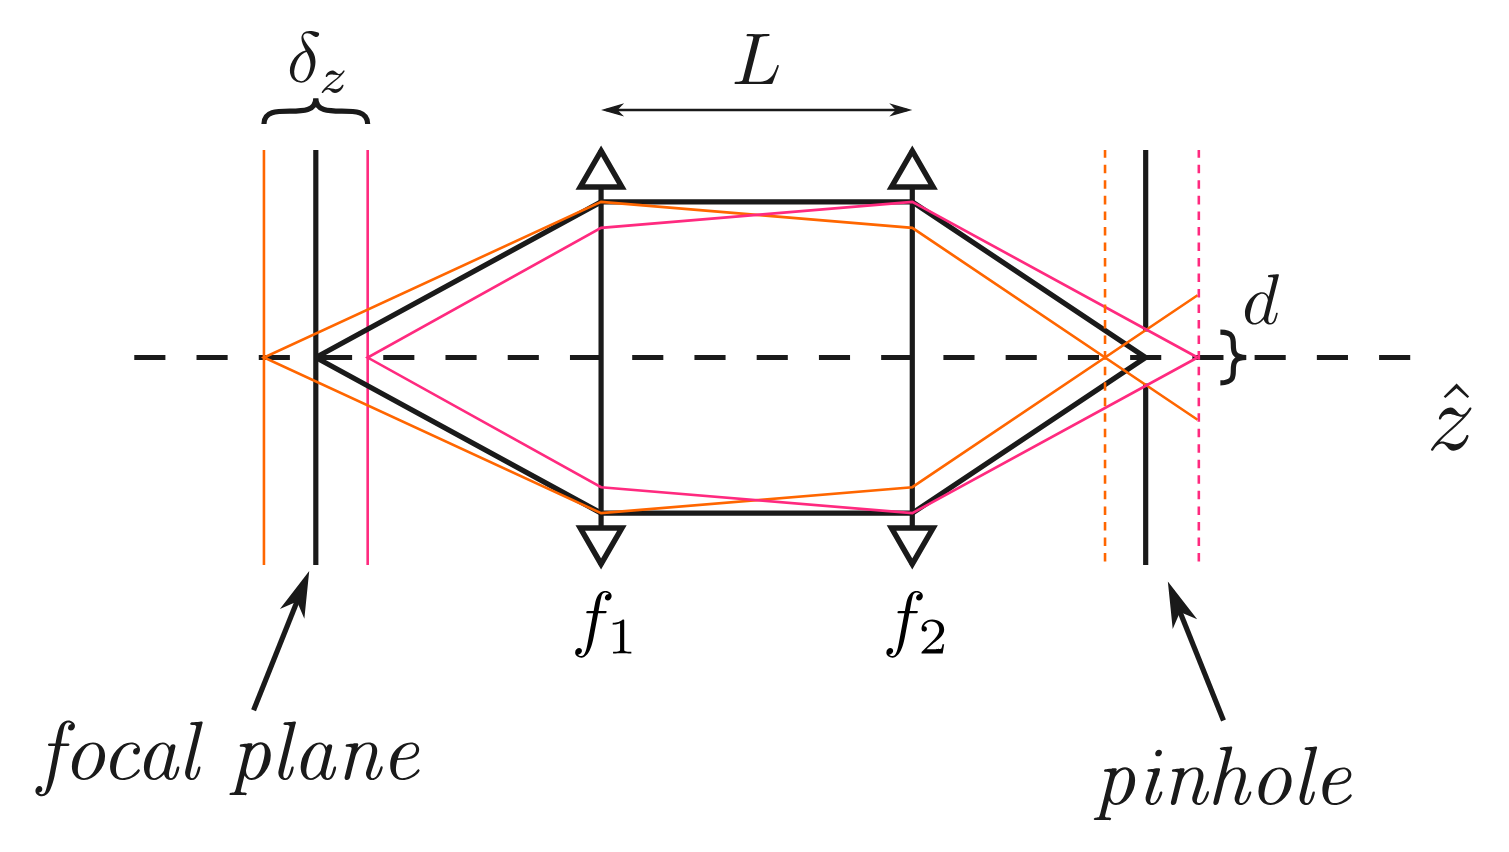
\includegraphics[scale=0.15]{rayons_pinhole.png}
  \caption{Schéma illustrant les rayons passant aux extrémités du sténopé}
  \label{rayons}
\end{figure}

À partir de ce schéma, il est possible de mettre le \textit{input plane} (IP), qui correspond à l'entrée des rayons lumineux, au plan focal, et le \textit{output plane} (OP), soit la sortie de ceux-ci, au sténopé. Ainsi, il est possible de poser une matrice de transfert $M$ au système de la façon suivante :

\begin{equation}
  M = M_{t3}M_{f2}M_{t2}M_{f1}M_{t1}
\end{equation}

où les matrices sont les suivantes :

\begin{itemize}
\item $M_{t1}$ est la matrice de translation entre le plan focal et la lentille 1
\item $M_{f1}$ est la matrice de lentille mince de la lentille 2
\item $M_{t2}$ est la matrice de translation entre les deux lentilles
\item $M_{f2}$ est la matrice de lentille mince de la lentille 2
\item $M_{t3}$ est la matrice de translation entre le plan focal et la lentille 1
\end{itemize}

Une matrice de translation se décrit par :

\begin{equation}
  M_{t}= 
  \begin{bmatrix}
    1 & x \\
    0 & 1
  \end{bmatrix}
\end{equation}

où $x$ est la longueur de la translation selon l'axe optique. Un matrice de lentille mince se décrit par :

\begin{equation}
  M_{f} = 
  \begin{bmatrix}
    1 & 0 \\
    -\frac{1}{f} & 1
  \end{bmatrix}
\end{equation}

où $f$ est la distance focale de la lentille. Soit $r_i$, un rayon de lumière initial au plan focal. Ce dernier se décrit par sa hauteur et par son angle par rapport à l'axe optique $\hat{z}$ :

\begin{equation}
  r_{i}= 
  \begin{bmatrix}
    y_{i} \\
    \alpha_{i}
  \end{bmatrix}= 
  \begin{bmatrix}
    0 \\
    \alpha_{i}
  \end{bmatrix}
\end{equation}

La hauteur $y_{i}$ est nulle car le rayon de lumière commence sur l'axe optique. Soit aussi $r_{f}$, le rayon final qui arrive au sténopé :

\begin{equation}
  r_{f}= 
  \begin{bmatrix}
    y_{f} \\
    \alpha_{f}
  \end{bmatrix}
\end{equation}

C'est avec la définition de ce rayon final qu'il est possible de développer le modèle pour la résolution axiale $\delta_{z}$. En effet, tel que visible à la figure \ref{rayons}, deux rayons finaux peuvent être dessinés à partir des deux extrémités du sténopé. Ces deux derniers convergent à des plans focaux qui ont une distance différente avec la première lentille. La différence entre ces distances est la résolution axiale recherchée.

Soit le cas 1, où l'on dénote la hauteur du rayon final au sténopé $y_{f1} = d/2$. Ce rayon est illustré en rouge. Il est possible de développer l'équation matricielle suivante :

\begin{align}
  r_{f1}&= M r_{i1}\label{matrixeq}\\
  \Rightarrow\begin{bmatrix}
    \frac{d}{2}  \\
    \alpha_{f1}
  \end{bmatrix} &= 
  M \begin{bmatrix}
    y_{i1} \\
    \alpha_{i1}
  \end{bmatrix}
\end{align}

L'angle $\alpha_{f1}$ se trouve par trigonométrie :

\begin{equation}
  \alpha_{f1}= \arctan\left( \frac{\phi_{f_{2}}-d}{2f_{2}} \right)
\end{equation}

où $\phi$ dénote le diamètre d'une lentille. Il est possible de dénoter la distance inconnue entre le plan focal du cas 1 et la lentille 1 par $z_{1}$. Cette dernière se trouve dans $M_{t1}$, et donc dans $M$. Du coup, à l'aide de la librairie de calcul symbolique \textit{sympy}, il est possible de calculer aisément la matrice de transfert et de résoudre l'équation (\ref{matrixeq}) avec la méthode \texttt{LUSolve}. Le résultat a donc la forme suivante :

\begin{equation}
  r_{i1}= \begin{bmatrix}
   y_{i1}(z_{1})  \\
    \alpha_{i1}(z_{1})
  \end{bmatrix}
\end{equation}

Or, sachant que :

\begin{equation}
  y_{i1}(z_{1})=0
\end{equation}

La fonction sympy \texttt{solve} permet de résoudre cette équation symboliquement pour $z_{1}$, et après substitution, sa valeur numérique peut être connue.

Ces étapes de résolution se répètent pour le cas 2, où l'on dénote la hauteur du rayon final au sténopé $y_{f2} = -d/2$. Ce rayon est illustré en orange. Son angle se trouve également par trigonométrie :

\begin{equation}
  \alpha_{f1}= \arctan\left( \frac{\phi_{f_{2}}+d}{2f_{2}} \right)
\end{equation}

Il est donc possible en résolvant les mêmes équations mais pour le cas 2 d'obtenir $z_{2}$. Enfin, la résolution axiale se trouve ainsi :

\begin{equation}
  \delta_{z}= |z_{2}-z_{1}|
\end{equation}

Cette valeur dépend donc de $z$, qui, à son tour, dépend des paramètres du montage physique.

\section{Méthodologie}

\section{Méthodologie}

La méthode utilisée lors de ce laboratoire à pour but de : mesurer l'impact d'un sténopé sur la résolution axiale ($\delta x$) d'un montage optique confocal. Ou en d'autre termes d'étbalir la relation entre la puissance du système et la position d'un objet observé avec et sans sténopé. La figure \ref{montage} présente le montage optique confocal utilisé lors du laboratoire. 

\begin{figure}[H]
  \centering
  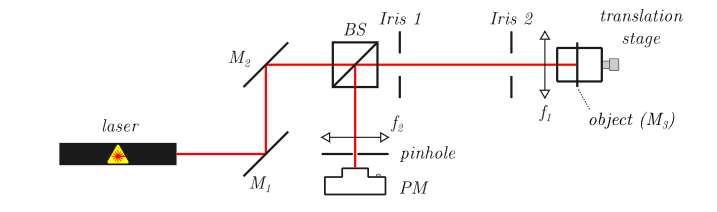
\includegraphics[scale=0.7]{Montage laboratoire 1.png}
  \caption{Montage optique confocal utilisé lors du laboratoire}
  \label{montage}
\end{figure}

Le matériel utilisé dans ce montage est :

\begin{itemize}
    \item[$-$]  1 source laser et source d’alimentation
    \item[$-$]  3 miroirs avec vis d’alignement ($M_i$)
    \item[$-$]  1 cube beam splitter ($BS$)
    \item[$-$]  2 iris (pour alignement)
    \item[$-$]  2 lentilles ($f_1 = f_2 = 35 mm, \phi_1 = \phi_1 = 25.4 mm$)
    \item[$-$]  1 stage de translation (\hat{z})
    \item[$-$]  1 monture de translation XY (\textit{thorlabs ST1XY-S(/M)})
    \item[$-$]  1 sténopé ($\phi = 75μm$)
    \item[$-$]  1 power meter ($PM$)
\end{itemize}

Dans ce système, l'objet observé ($M_s$) est un miroir. Sa fonction est de réfléchir un rayon émit depuis une source laser, puis filtré en longueur d'onde par des miroir dichroïques ($M1$ et $M2$), vers un puissance-mètre ($PM$). Ce rayon est focalisé une première fois par une lentille ($f_1$) puis redirigée après reflexion vers une autre lentille ($f_2$) afin de mesurer l'impact du déplacement du miroir sur la puissance mesurée. Cette partie du montage correspond au système optique présenté dans la figure \ref{rayons} et peut donc être décrit par les équations développées dans la partie théorie. Le miroir est rendu mobile par une monture de translation et la déviation vers la seconde lentille se fait par l'intermédiare d'un "cube beam splitter" ($BS$). \\

De façon concrête, le but des expériences est de placer le miroir à une position focalisé, où la puissance captée est maximale, puis de le faire bouger selon l'axe de translation du faisceaux. Cette démarche permet de récolter un paquet de données, permettant grâce à une interpolation d'établir la relation entre la puissance et la position du capteur. En répétant ce même protocole deux fois sur des montages similaires, d'abord sans le sénopé, puis avec, les relations établies permettent de comprendre son impact vis-à-vis de la distance focale du système ($\delta x$). 

\section{Hypothèses}

Afin de prédire le comportement de la résolution axiale en fonction des différents paramètres physiques du système, un modèle de calcul ainsi qu'un programme python a été utilisé. Ces derniers sont présentés en annexe. Le programme python utilise d'abord la librairie numpy afin de définir des fonctions qui génèrent des matrices de translation ou de lentille mince. Ensuite, une fonction est créée pour calculer la résolution axiale en fonction de la largeur du sténopé, de la distance focale ainsi que de la distance séparant les lentilles, tel que décrit dans le modèle de calcul. Dans cette fonction, sympy est utilisé pour effectuer la résolution symbolique de la multiplication matricielle et des équations autant algébriques que matricielle. À la fin de cette fonction, les valeurs numériques sont substituées pour avoir une valeur numérique de résolution. Le programme utilise enfin matplotlib afin de de visualiser le résultat de cette fonction pour des plages de paramètres.

Le graphique présenté en figure \ref{respin} démontre la variation de la résolution axiale pour une plage de diamètre de sténopé et ce, pour cinq valeurs différentes de longueur focale.

\begin{figure}[H]
  \centering
  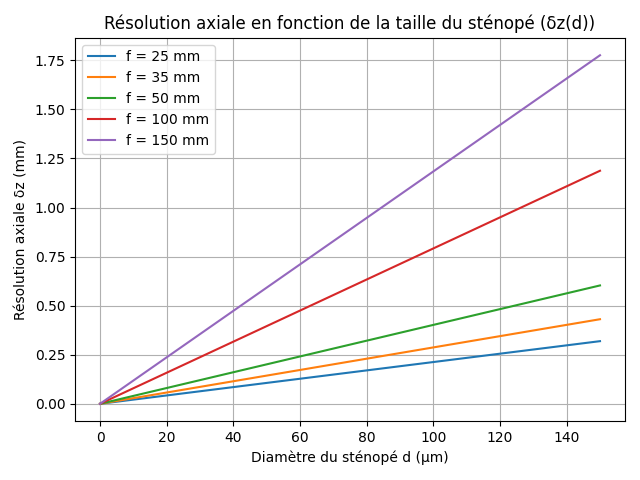
\includegraphics[scale=0.7]{res_vs_pinhole.png}
  \caption{Graphique de $\delta_{z}$ en fonction de $d$ pour différentes valeurs de $f$.}
  \label{respin}
\end{figure}
''
L'hypotèse présentée par le modèle de calcul est que la variation de $d$ fait augmenter linéairement la résolution axiale. Ensuite, la figure \ref{resfoc} montre la variation de la résolution axiale pour une plage de longueur focale des deux lentilles, pour quatres valeurs différentes de diamètre de sténopé.
\begin{figure}[H]
  \centering
  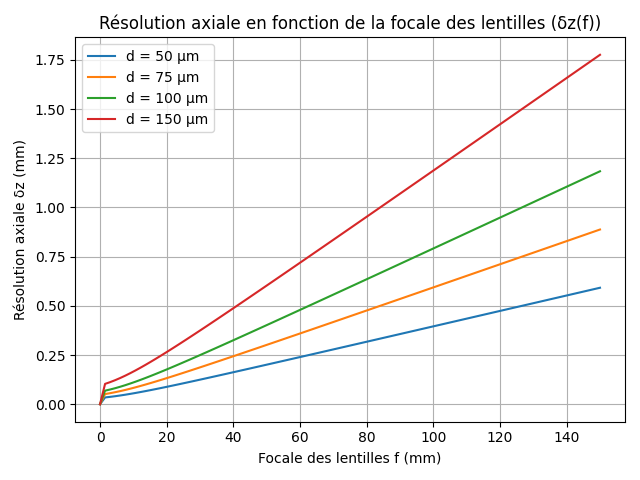
\includegraphics[scale=0.7]{res_vs_focal.png}
  \caption{Graphique de $\delta_{z}$ en fonction de $f$ pour différentes valeurs de $d$.}
  \label{resfoc}
\end{figure}

Il est donc possible de prédire un comportement quasi-linéaire pour la résolution axiale en fonction de la focale. Ce comportement ne semble toutefois pas valide pour des valeurs de $f$ très petites. Enfin, la figure \ref{resl} présente la résolution axiale en fonction de la distance entre les lentilles pour cinq valeurs différents de focales. 

\begin{figure}[H]
  \centering
  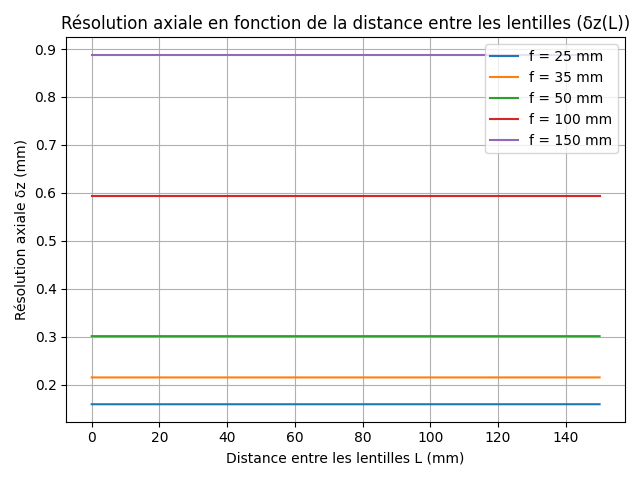
\includegraphics[scale=0.7]{res_vs_L.png}
  \caption{Graphique de $\delta_{z}$ en fonction de $L$ pour différentes valeurs de $f$.}
  \label{resl}
\end{figure}

L'hypothèse finale tirée du modèle est donc que la variation de $L$ n'a pas d'impact sur la résolution. 

\section{Annexes}

\subsection{Code source}

\begin{lstlisting}[language=python]
import numpy as np
import matplotlib.pyplot as plt
import sympy as sp

def Mt(d):
    '''Translation'''
    M = np.array([[1, d],
                  [0, 1]])
    return M

def Ml(f):
    '''Thin Lens'''
    M = np.array([[1, 0],
                  [-1/f, 1]])
    return M

def res_axial(pinhole, focal, lens_distance):
    """
    Calcule la resolution axiale en fonction du diametre du trou, de la focale, et de la distance entre les lentilles.

    Parametres :
    ------------
    pinhole : float
        Diametre du trou en metres.
    focal : float
        Longueur focale de la lentille en metres.
    lens_distance : float
        Distance entre les lentilles en metres.

    Retour :
    --------
    res : expression symbolique
        La resolution axiale en metres.
    """
    f = sp.symbols('f')
    phi = sp.symbols('phi')
    d = sp.symbols('d')
    L = sp.symbols('L')
    z = sp.symbols('z')

    # formation de la matrice de transfert
    M = Mt(f)@Ml(f)@Mt(L)@Ml(f)@Mt(z)
    M_sp = sp.Matrix(M)

    # definition des hauteurs et angles de chaque cote du pinhole
    yf1 = d/2
    alphaf1 = -sp.atan((phi-d)/(2*f))
    
    yf2 = -d/2
    alphaf2 = -sp.atan((phi+d)/(2*f))

    # vecteur decrivant le rayon final au pinhole
    vf1 = sp.Matrix([yf1, alphaf1])
    vf2 = sp.Matrix([yf2, alphaf2])

    # resolution des systemes matriciels puis de leur 1re 
    # equation = 0 pour isoler z
    solve1 = M_sp.LUsolve(vf1)
    z1 = sp.solve(solve1[0], z)

    solve2 = M_sp.LUsolve(vf2)
    z2 = sp.solve(solve2[0], z)

    # substitution des valeurs numeriques
    values = {f:focal, phi:25.4e-3, d:pinhole, L:lens_distance}
    res = z2[0].subs(values) - z1[0].subs(values)

    return res

# set de courbes 1
focals = [25e-3, 35e-3, 50e-3, 100e-3, 150e-3]
pinhole_sizes = np.linspace(0, 150e-6, 100)
L = lambda f: f

plt.figure()

# Tracer une courbe pour chaque focale
for f in focals:
    res_values = [res_axial(d, f, L(f)) * 1e3 for d in pinhole_sizes]
    plt.plot(pinhole_sizes * 1e6, res_values, label=f'f = {f*1e3:.0f} mm')

# Parametres d'affichage
plt.xlabel("Diametre du stenope d (micro m)")
plt.ylabel("Resolution axiale delta z (mm)")
plt.legend()
plt.grid(True)
plt.title("Resolution axiale en fonction de la taille du stenope (dz(d))")
plt.tight_layout()
plt.savefig("res_vs_pinhole.png")
plt.show()
plt.clf()

# set de courbes 2
pinhole_sizes = [50e-6, 75e-6, 100e-6, 150e-6]
focals = np.linspace(1e-6, 150e-3, 100)
L = lambda f: f  # si L(f) appele, L = f

plt.figure()

# Tracer une courbe pour chaque taille de stenope
for pinhole in pinhole_sizes:
    res_values = [res_axial(pinhole, f, L(f)) * 1e3 for f in focals]
    plt.plot(focals * 1e3, res_values, label=f'd = {pinhole*1e6:.0f} micro m')

# Parametres d'affichage
plt.xlabel("Focale des lentilles f (mm)")
plt.ylabel("Resolution axiale dz (mm)")
plt.legend()
plt.grid(True)
plt.title("Resolution axiale en fonction de la focale des lentilles (dz(f))")
plt.tight_layout()
plt.savefig("res_vs_focal.png")
plt.show()
plt.clf()

# set de courbes 3
pinhole = 75e-6  # 75 micro m
focals = [25e-3, 35e-3, 50e-3, 100e-3, 150e-3]  # en metres
lens_distances = np.linspace(0, 150e-3, 100)  # en metres

plt.figure()

# Tracer une courbe pour chaque taille de focale
for f in focals:
    res_values = [res_axial(pinhole, f, L) * 1e3 for L in lens_distances]
    plt.plot(lens_distances * 1e3, res_values, label=f'f = {f*1e3:.0f} mm')

# Parametres d'affichage
plt.xlabel("Distance entre les lentilles L (mm)")
plt.ylabel("Resolution axiale dz (mm)")
plt.legend()
plt.grid(True)
plt.title("Resolution axiale en fonction de la distance entre les lentilles (dz(L))")
plt.tight_layout()
plt.savefig("res_vs_L.png")
plt.show()
plt.clf()
\end{lstlisting}



\clearpage

% \bibliographystyle{unsrtnat}
% \bibliography{My_Library}

\end{document}
